\documentclass{article}

% Language setting
% Replace `english' with e.g. `spanish' to change the document language
\usepackage[english]{babel}

% Set page size and margins
% Replace `letterpaper' with `a4paper' for UK/EU standard size
\usepackage[letterpaper,top=2cm,bottom=2cm,left=3cm,right=3cm,marginparwidth=1.75cm]{geometry}

% Useful packages
\usepackage{amsmath}
\usepackage{graphicx}
\usepackage{float}
\usepackage[colorlinks=true, allcolors=blue]{hyperref}

\title{BP CRM - Practical Assessment Devsu - Solution Architect}
\author{Alejandro Ferrante}

\begin{document}
\maketitle


El objetivo de este documento es presentar una estructura de tipo C4 que describa una posible solución de diseño para la implementación del sistema planteado en la consigna proporcionada. Se asumió en todo momento que el CRM a implementar se realizaría utilizando la tecnología Salesforce.
\newline \newline

\begin{figure} [H]
\centering
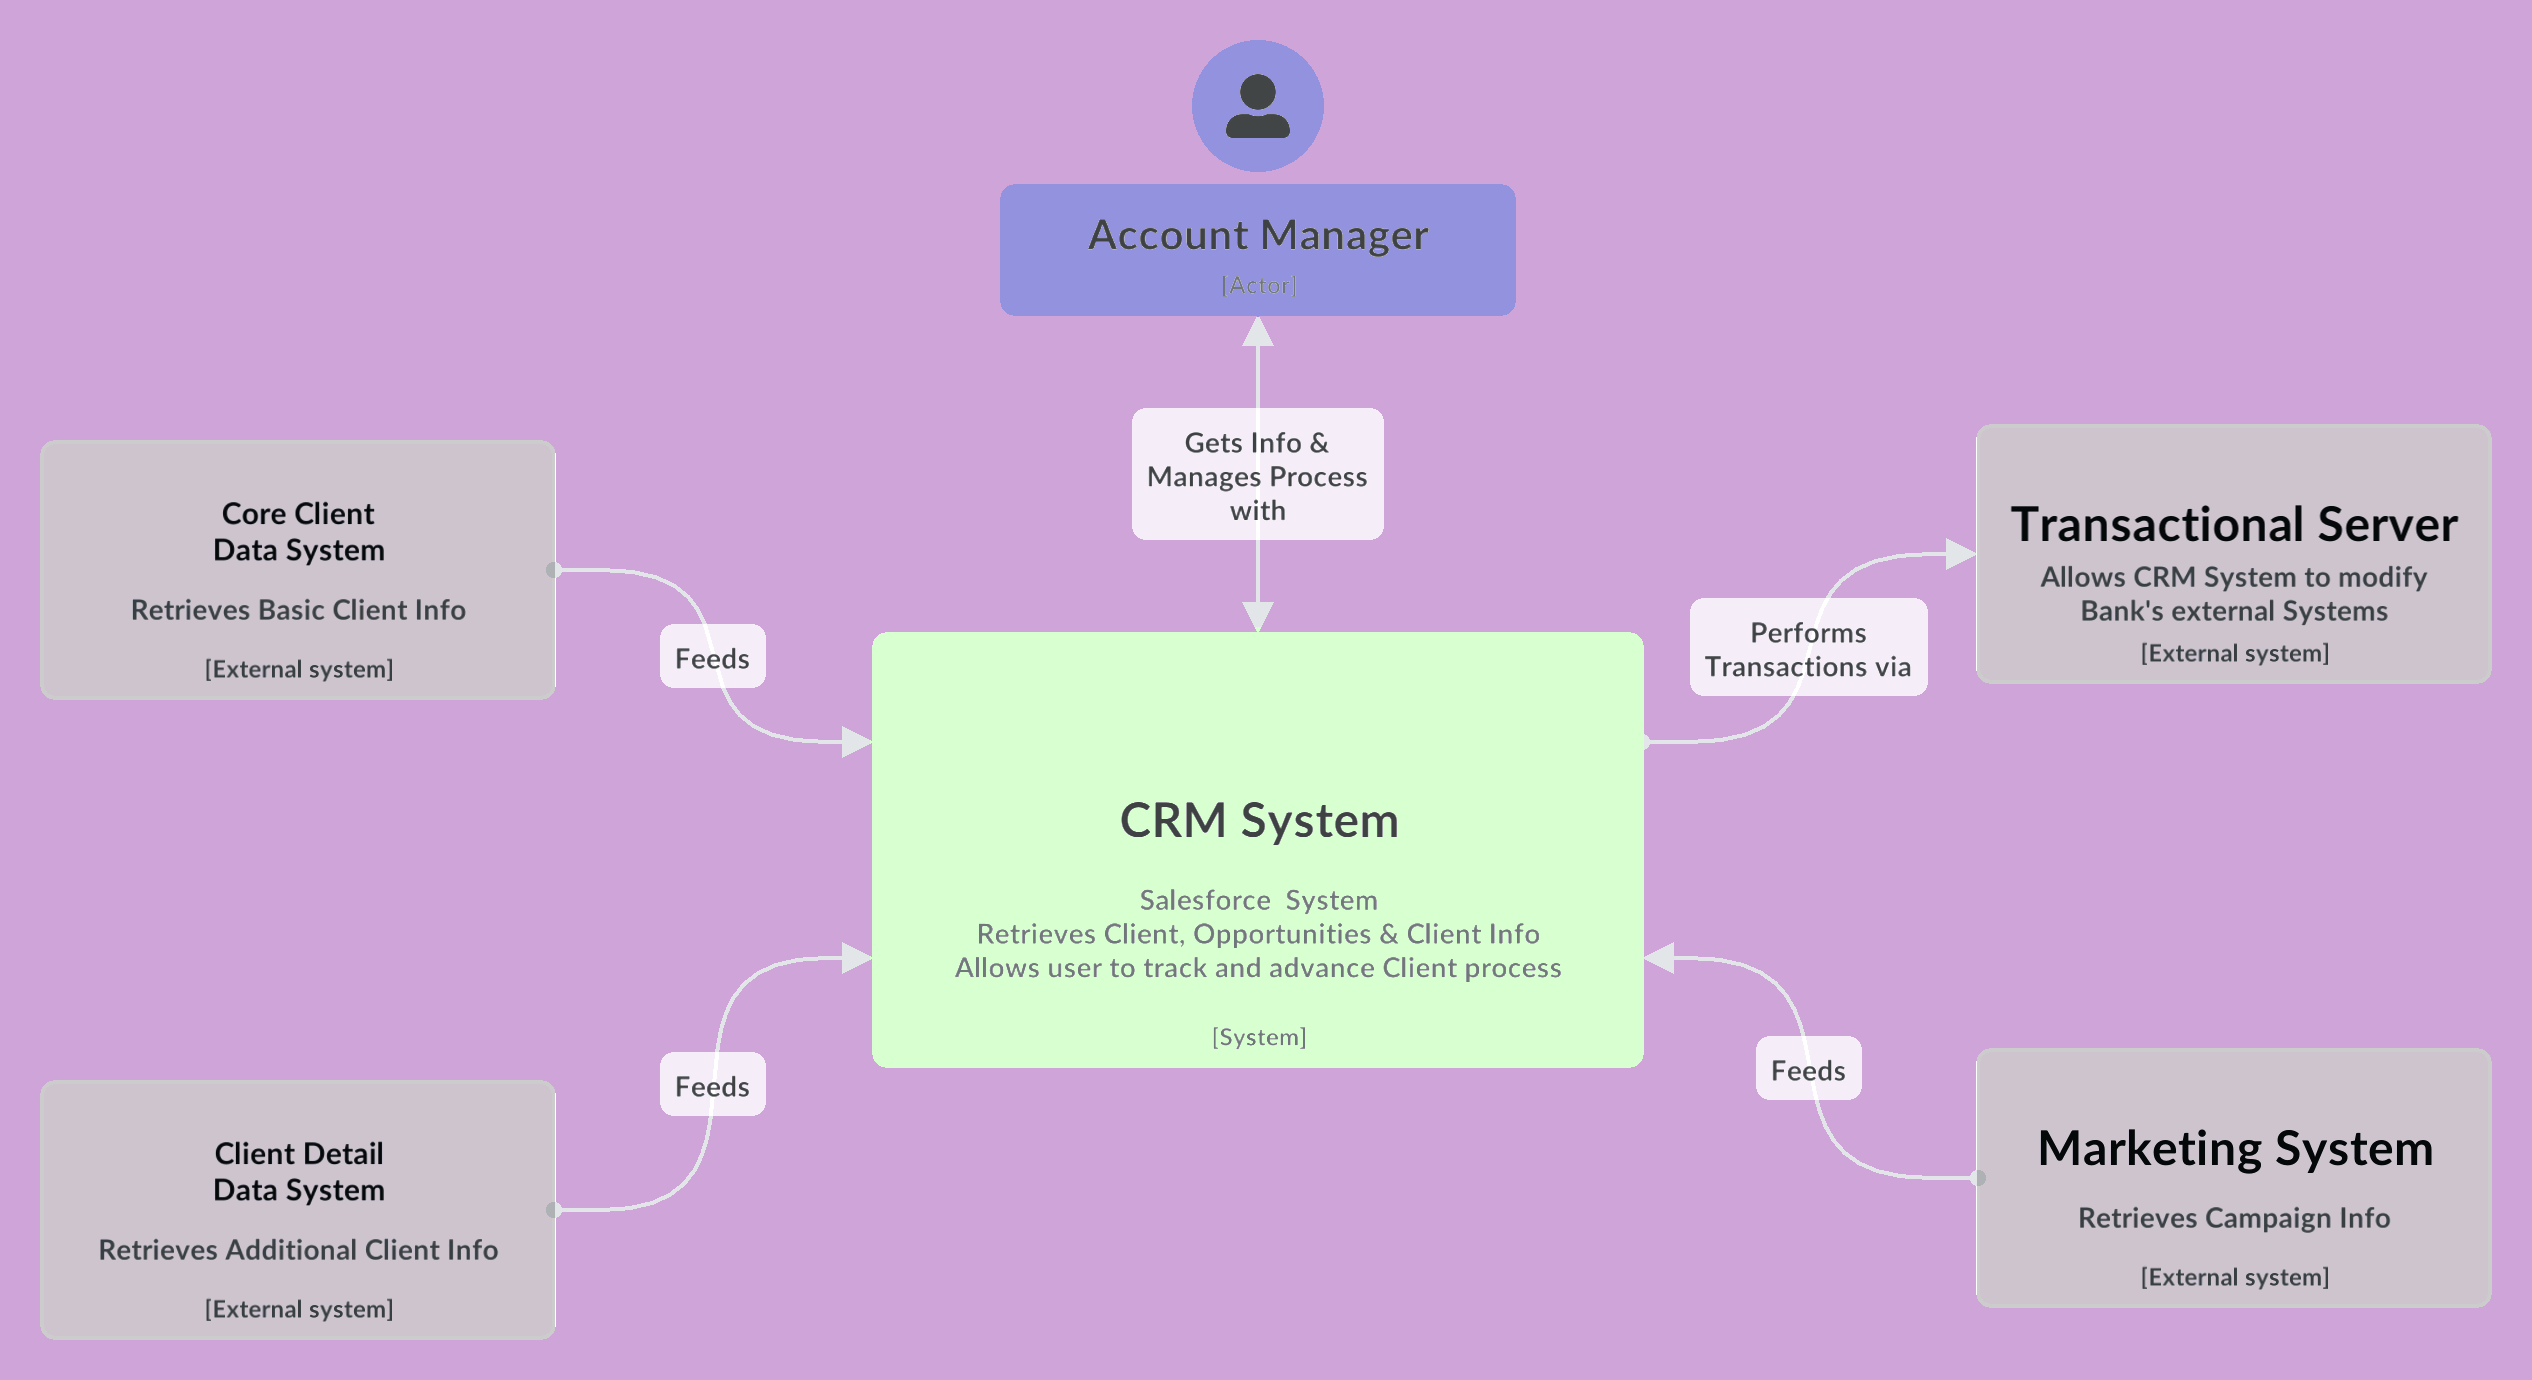
\includegraphics[width=0.9\linewidth]{C1 Context.png}
\caption{\label{fig:C1}Nivel 1: Diagrama de Contexto.}
\end{figure}

\begin{figure} [H]
\centering
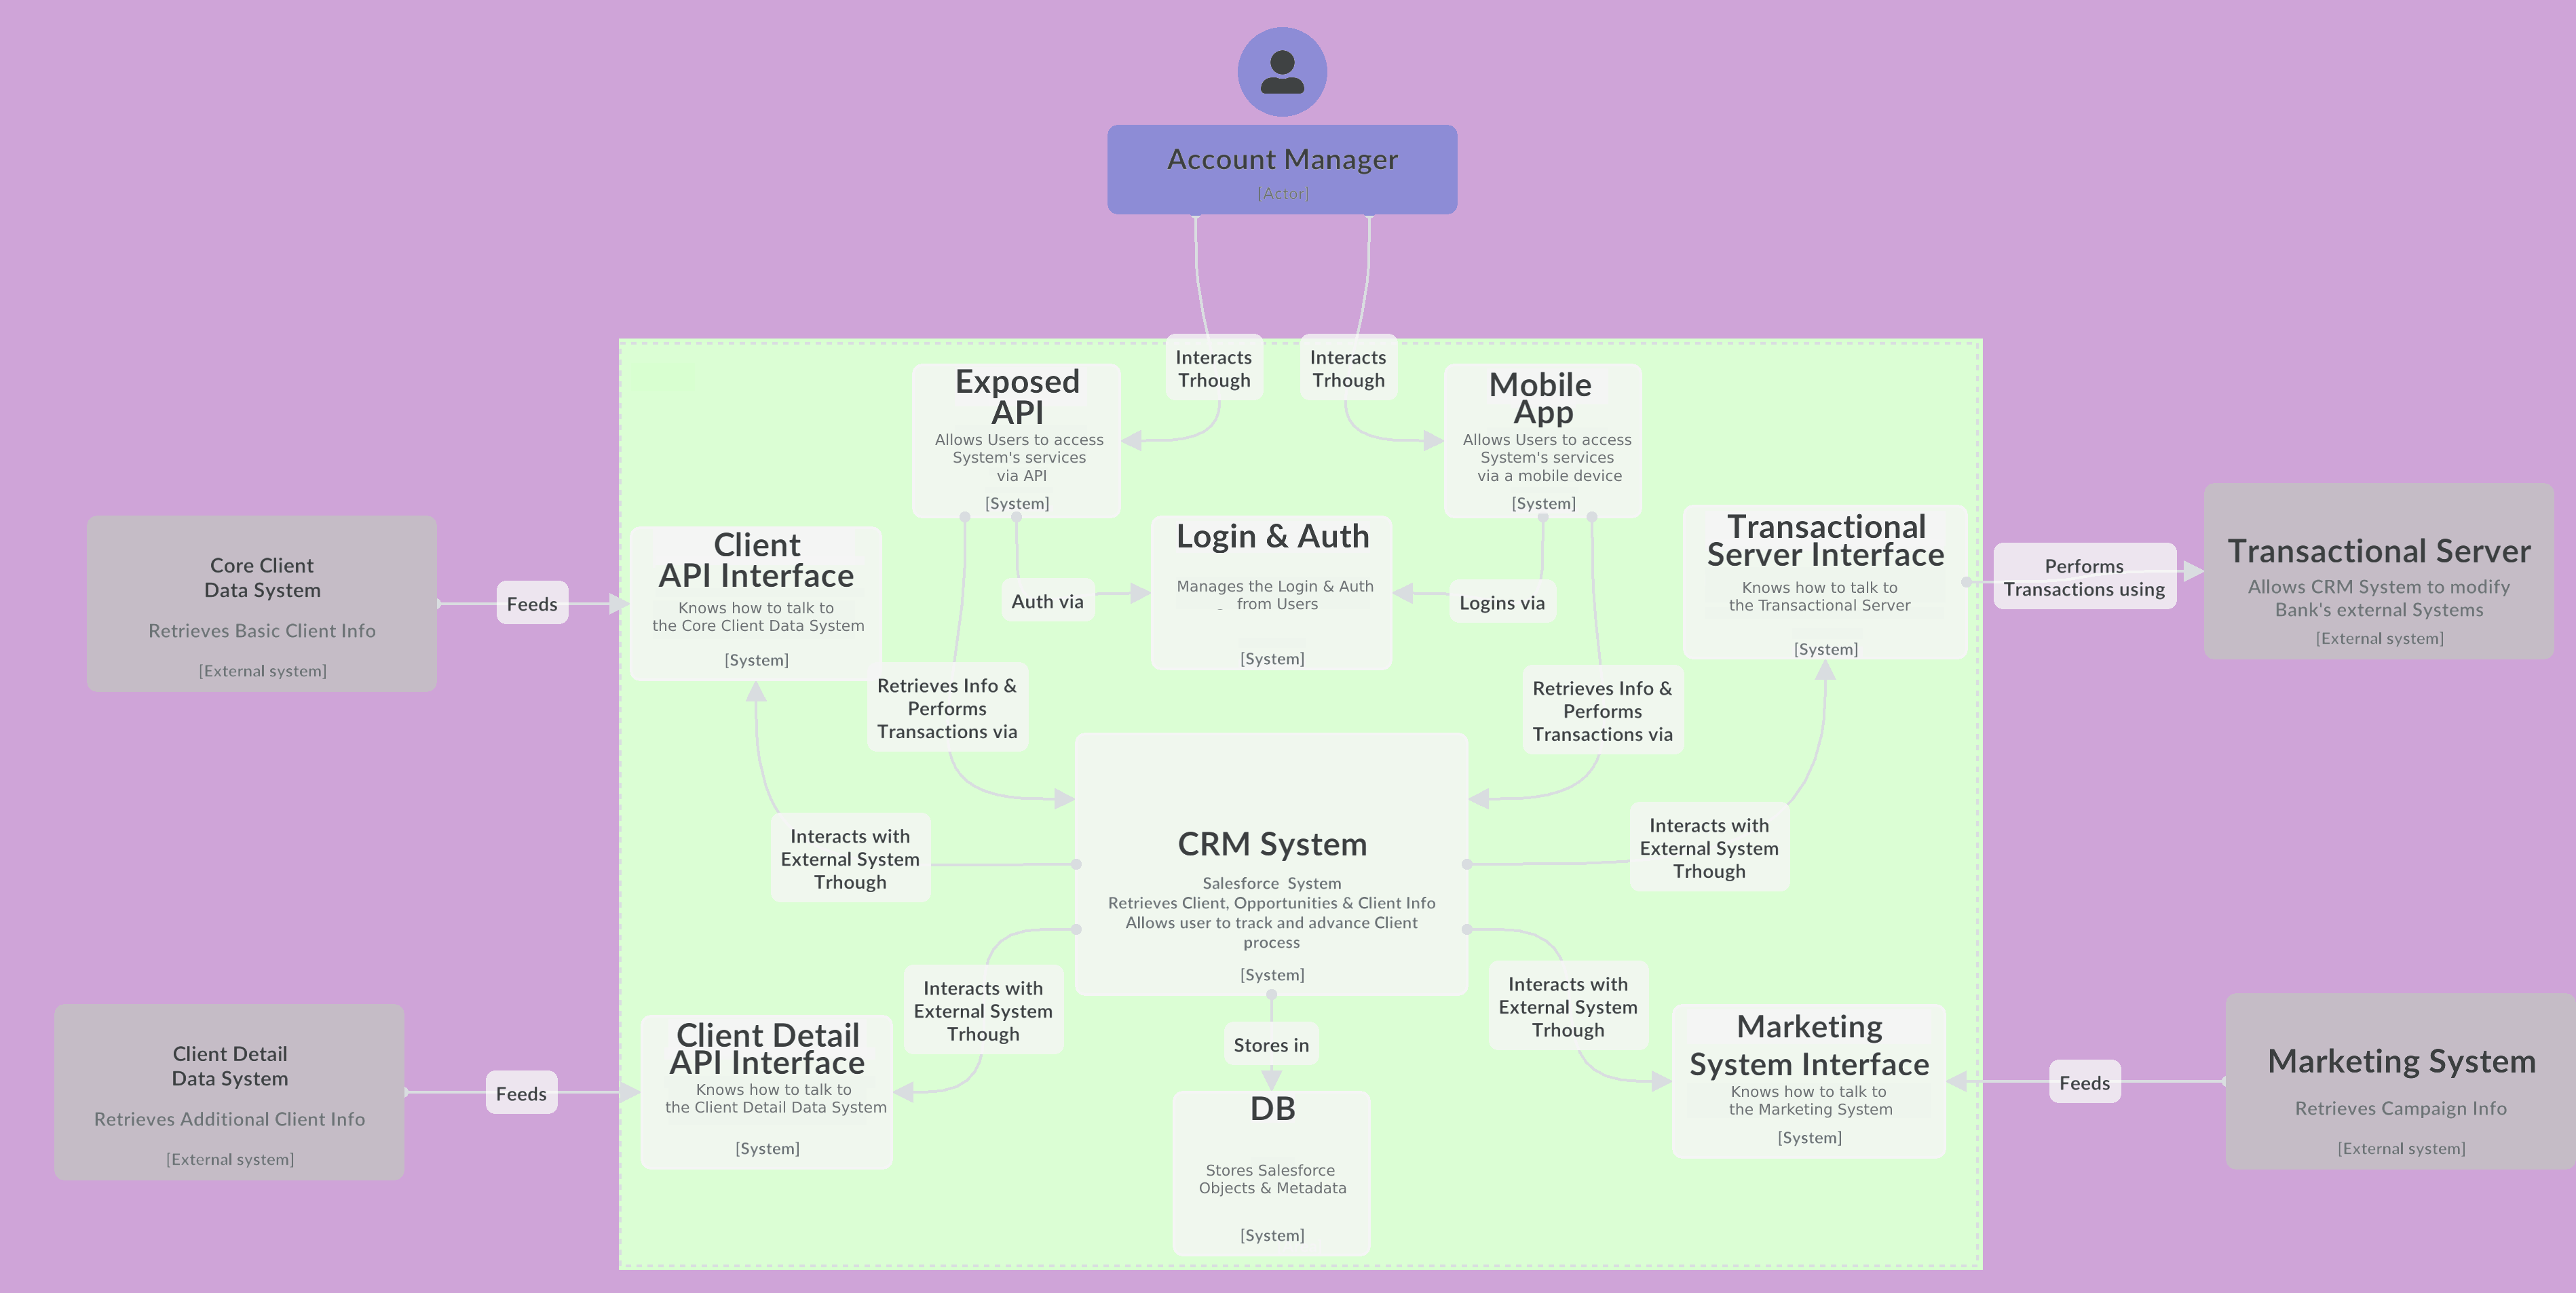
\includegraphics[width=0.9\linewidth]{C2 Containers.png}
\caption{\label{fig:C2}Nivel 2: Diagrama de Contenedores.}
\end{figure}

Las figuras \ref{fig:C1} y \ref{fig:C2} muestran los esquemas correspondientes a los primeros dos niveles: El primero según la estructura C4 es el Contexto, mientras que el segundo es el de contenedores.\footnote{Nota: No se especificó en la consigna pero se asume que la información a cerca de los casos de soporte provienen de alguno de los sistemas externos ilustrados en los diagramas.}
\newline \newline
En cuanto al tercer nivel, se entiende que por la característica de este ejercicio se proporciona una descripción general del problema. Es por esto que śiempre habrá información no explicitada.
Sin embargo, esta información (en particular la referente al funcionamiento de los sistemas externos) es necesaria a la hora de tomar decisiones de diseño a mas bajo nivel. Adicionalmente, al el sistema estar basado en Salesforce, muchos componentes de la herramienta son preexistentes e inamovibles. Se pueden incluir en los diagramas de nivel 3, pero no se posee decisión sobre su composición.
Es por esta razón que al no poder tomar decisiones certeras no se pueden materializar en diagramas de nivel 3.
\newline \newline
A la hora de diseñar, hacer las preguntas correctas a las personas correctas es tan importante como poder comunicar efectivamente las decisiones y el diseño a cada tipo de participante en el proceso.
A continuación, se discuten algunas preguntas que se podrían hacer para orientar decisiones de diseño y aplicación de distintos patrones. Cada una de estas secciones se discutiría con los stakeholders correspondientes para llegar a una decisión que satisfaga a todas las partes.

\section{Seguridad}

Dado el contexto del tipo de sistema a implementar, resulta claro que este debe poseer un nivel de seguridad superior al que podrían requerir otro tipo de soluciones. Es por esto que resulta indispensable hacer uso de la mayor cantidad de opciones de las cuales la plataforma Salesforce nos provee.
\newline \newline
Esto incluye el paquete de funcionalidades Salesforce Shield, Privacy Center, Data Masking y Audit Trail.

Salesforce Shield provee tres capacidades principales: Event Monitoring, Field Audit Trail y Platform Encryption.
Esto se traduce a una mayor capacidad de monitoreo de la actividad y los cambios en la plataforma (que se complementa con el mecanismo de Audit Trail), además de la capacidad de encriptar los datos sensibles.
\newline \newline
En concordancia con la encriptación de datos sensibles, el uso de Data Mask permite que los datos utilizado en los ambientes Sandbox sean enmascarados para no reflejar al cien porciento sus contrapartes en los ambientes de producción, sin afectar el volumen de datos disponibles en este tipo de ambiente.
\newline \newline
En esta etapa será sumamente importante recolectar información a cerca de las regulaciones y estándares de seguridad necesarios para el sistema propuesto. Salesforce cuenta con Privacy Center, una herramienta que esta diseñada para ayudar específicamente con ese tipo de cuestiones.
\newline \newline
Finalmente, una medida de seguridad imprescindible es el de la implementación de una autenticación en varias etapas, o MFA para evitar accesos indeseados al sistema.
\newline \newline
Las figuras \ref{fig:MFA} y \ref{fig:PrivCenter} muestran lo que podría ser parte de la presentación para la reunión de stakeholders.

\begin{figure} [H]
\centering
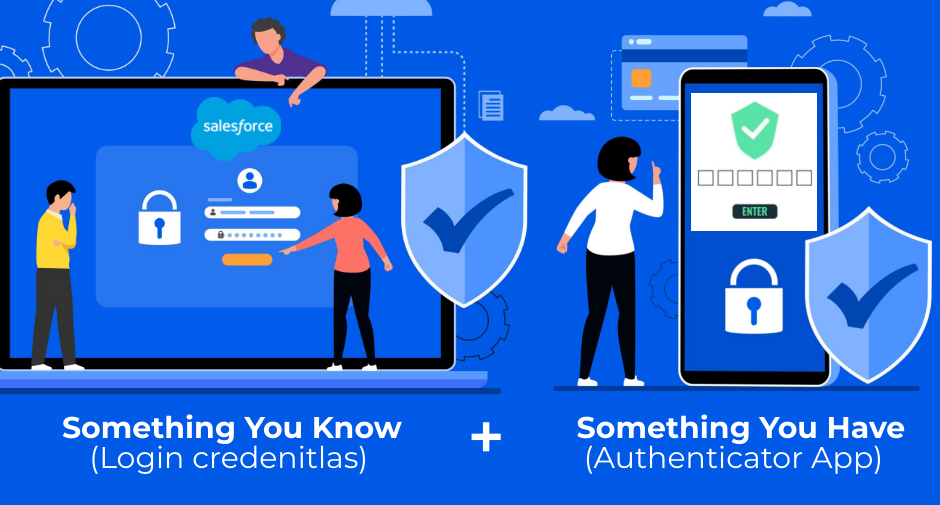
\includegraphics[width=0.5\linewidth]{MFA.png}
\caption{\label{fig:MFA}Slide: Multi Factor Authentication.}
\end{figure}

\begin{figure} [H]
\centering
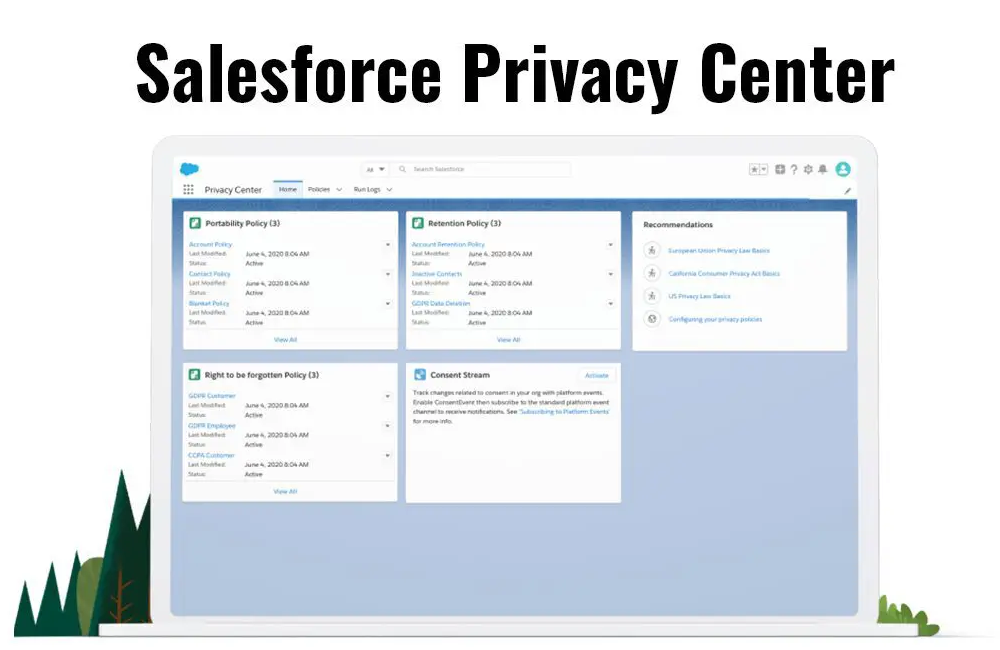
\includegraphics[width=0.5\linewidth]{Privacy Center.png}
\caption{\label{fig:PrivCenter}Slide. Salesforce Privacy Center.}
\end{figure}

\section{Login}

Siguiendo con el ultimo punto a cerca de MFA, se puede discutir otros aspectos del login del sistema, como lo es el single sign on (SSO). Las ventajas generales están relacionadas con la simplicidad y practicidad, aunque crea un punto de dependencia externa para el proceso de login y potencialmente un punto único de fallo (Single Point of Failure). Inicialmente no lo consideraría necesario a menos que el mismo mecanismo ya este siendo utilizado por los usuarios para aplicaciones similares.


\section{Aplicación Móvil}

La descripción inicial menciona que uno de las dos formas de interactuar con el sistema sea a través de una aplicación móvil. 
\newline \newline
Esto nos presenta con una dicotomía básica de si desarrollar una aplicación  personalizada o utilizar la funcionalidad nativa de Salesforce Mobile. Esta pregunta encierra por detrás otra mas interesante que afecta no solo a la aplicación móvil, sino a todo el sistema: ¿Debería utilizarse la funcionalidad estándar de Salesforce o construir sobre la plataforma una aplicación custom?
\newline \newline
La regla general es ``no reinventar la rueda'' y siempre intentar hacer el mayor uso de las capacidades ya existentes de Salsforce (esto podría no ser suficiente si ya existen otros sistemas similares y se busca cierta integridad visual que no puede ser satisfecha nativamente) antes de encarar un desarrollo custom (programación Apex, Visualforce, NodeJs, ReactJs, etc.).
\newline \newline
Por la descripción inicial, parece que se manejaran objetos ya existentes en Salesforce (Clientes, Cuentas, Oportunidades, Campañas, etc.), por lo que probablemente la funcionalidad estándar sea suficiente para cubrir los requerimientos. 
\newline
En tándem con esta decisión, la aplicación móvil podría ser la de Salesforce Mobile, que proporciona una buena experiencia para el uso estándar de la plataforma. Otros factores relevantes es si se cuenta con el tiempo, presupuesto o incluso expertise para desarrollar dicha aplicación.

\section{Almacenamiento e Integración}

Siguiendo con el razonamiento anterior, resulta seguro asumir que pocos o ningún objeto custom será necesario para esta implementación.
\newline
Sin embargo, debemos preguntarnos a cerca de volumen de datos manejados por los sistemas externos y la naturaleza de los mismos.
Tratándose de objetos estándar podemos asumir que Salesforce puede almacenar los objetos necesarios (a excepción de las oportunidades, que requieren un análisis especial por tratarse de un gran volumen). 
\newline \newline
Sin embargo, almacenarlos en la base de datos de la org, si bien puede garantizarnos mayor rapidez y confiabilidad a la hora de consultarlos, introduce redundancia de datos. Esto significa que si una oportunidad por ejemplo cambia en un sistema externo, este cambio debe reflejarse en la org. Analogamente, si un cambio es hecho en la org, debe ser reflejado en los sistemas externos que corresponda (sabemos que esto se hace a través del sistema de Transacciones). 
\newline \newline
En el caso que no sean almacenados en la org, las dos estrategias principales consisten en utilizar Salesorce Connect y Remote Objects, mapeando los objetos del sistema externo a objetos virtuales en Salesforce que pueden ser manipulados, o obtener la información on demand con el llamado a cada sistema (esto ultimo puede traer problemas con volúmenes de datos muy grandes).
\newline \newline
En el caso de ser almacenados en la org, se puede optar por trabajos programados de data loading fuera del horario de operaciones, o una solución basada en eventos como lo es la Streaming API, donde se puede suscribir al evento de creación o modificación de un registro reflejándolo en la base de datos.
Cabe destacar que distintas estrategias pueden ser utilizadas para distintos objetos dependiendo de su naturaleza.
\newline \newline
Tambien debe explorarse la posibilidad de utilizar un servicio de integración como puede ser Mulesoft.
\newline \newline
Finalmente, una pregunta básica es el tipo de API que se utiliza en cada caso (si es REST o SOAP), el volumen de datos que maneja y su confiabilidad. Esto ultimo vendrá aparejado con el diseño de un plan de contingencia en caso de que alguno de los servicios se encuentre no disponible.





\end{document}